% !TEX program = xelatex
\documentclass[a4paper,12pt]{article}

\usepackage{fontspec}
\usepackage{microtype}
\usepackage{graphicx}
\usepackage{booktabs}
\usepackage{longtable}
\usepackage{xcolor}
\usepackage{fancyvrb}
\usepackage[a4paper,margin=2.2cm]{geometry}
\usepackage[unicode=true,colorlinks=true,linkcolor=black,citecolor=black,
            urlcolor=black,bookmarksnumbered=true]{hyperref}
\usepackage{bookmark}
\usepackage{xurl}

\usepackage{xepersian}

\IfFontExistsTF{Vazirmatn}{\settextfont[Ligatures=TeX]{Vazirmatn}}{%
  \IfFontExistsTF{Shabnam}{\settextfont[Ligatures=TeX]{Shabnam}}{%
    \IfFontExistsTF{Sahel}{\settextfont[Ligatures=TeX]{Sahel}}{%
      \IfFontExistsTF{Amiri}{\settextfont[Ligatures=TeX]{Amiri}}{%
        \settextfont[Ligatures=TeX]{DejaVu Sans}}}}}
\IfFontExistsTF{TeX Gyre Termes}{%
  \setlatintextfont{TeX Gyre Termes}}{%
  \IfFontExistsTF{Liberation Serif}{%
    \setlatintextfont{Liberation Serif}}{%
    \setlatintextfont{DejaVu Serif}}}
\IfFontExistsTF{Vazirmatn}{\setdigitfont{Vazirmatn}}{%
  \IfFontExistsTF{Shabnam}{\setdigitfont{Shabnam}}{%
    \IfFontExistsTF{Sahel}{\setdigitfont{Sahel}}{%
      \IfFontExistsTF{Amiri}{\setdigitfont{Amiri}}{%
        \setdigitfont{DejaVu Sans}}}}}
\IfFontExistsTF{TeX Gyre Cursor}{\setmonofont[Scale=0.92]{TeX Gyre Cursor}}{%
  \IfFontExistsTF{DejaVu Sans Mono}{\setmonofont[Scale=0.90]{DejaVu Sans Mono}}{%
    \setmonofont[Scale=0.90]{Liberation Mono}}}

\newcommand{\en}[1]{\lr{#1}}
\pdfstringdefDisableCommands{\def\lr#1{#1}\def\en#1{#1}}

\emergencystretch=2em
\setlength{\parskip}{0.4em}

\begin{document}

\title{تعریف اصطلاح‌ها با \en{HTML}}
\author{}
\date{}
\maketitle

\begin{abstract}
\en{HTML} چند راه برای نشان‌دادن معنای «توصیف» دارد؛ گاهی وسط جمله،
گاهی در یک واژه‌نامهٔ مرتب. در این مطلب می‌بینیم وقتی می‌خواهید یک
\en{keyword} را تعریف کنید، آن را در کدام نشانه بگذارید.
\end{abstract}

\section*{پیش‌نیاز و هدف}

\begin{description}
\item[پیش‌نیاز:] با ساخت یک سند سادهٔ \en{HTML} آشنا باشید.
\item[هدف:] یاد بگیرید \en{keyword} تازه را چطور معرفی کنید و
\en{description list} را چطور بسازید.
\end{description}

وقتی معنی واژه‌ای را ندانید، معمولاً به فرهنگ لغت یا واژه‌نامه سر
می‌زنید. آنجا \en{keyword} را رسمی به یک یا چند شرح وصل می‌کنند؛ مثلاً:

\begin{quote}
\textbf{\en{Blue} (صفت)}\\
رنگی شبیه آسمان در روز آفتابی.
\textit{«آسمان آبیِ صاف»}
\end{quote}

ولی در نوشته‌های روزمره همان کار را غیررسمی هم می‌کنیم؛ مثل این:

\begin{quote}
\textbf{\en{Firefox}} همان مرورگر وبی است که \en{Mozilla Foundation}
ساخته است.
\end{quote}

برای همین کارها، \en{HTML} چند \en{tag} دارد تا هم شرح را علامت بزنید و
هم واژه‌ای را که شرح می‌دهید. با این کار، خواننده بهتر می‌فهمد منظورتان
چیست.

\section{چطور توصیف غیررسمی را علامت بزنیم}

در کتاب درسی، بار اول که \en{keyword} می‌آید، اغلب آن را پررنگ می‌کنند و
همان‌جا معنایش را می‌نویسند.

در \en{HTML} هم تقریباً همین کار را می‌کنیم. ولی چون \en{HTML} برای ظاهر
صفحه نیست، به‌جای پررنگ‌کردن از \en{<dfn>} استفاده می‌کنیم. این
\en{element} فقط برای اولین جایی است که یک \en{keyword} می‌آید. مهم است
که \en{<dfn>} را دور خودِ واژه بگذارید، نه دور تعریف؛ تعریف همان
پاراگراف کامل است:

\begin{latin}
\begin{Verbatim}[fontsize=\small,frame=single,framesep=4pt]
<p><dfn>Firefox</dfn> is the web browser created by the Mozilla Foundation.</p>
\end{Verbatim}
\end{latin}

\begin{quote}
\textbf{توجه:} پررنگ‌کردن برای تأکید هم به کار می‌رود. خودِ «پررنگ» مفهومی
مربوط به ظاهر است و جای مستقیمی در \en{HTML} ندارد؛ ولی برای تأکید،
\en{tag}های جداگانه‌ای هست.
\end{quote}

\section{حالت خاص: مخفف‌ها}

مخفف را بهتر است با \en{<abbr>} جدا علامت بزنید تا \en{screen reader}
درست بخواندش و خودتان هم بتوانید روی همهٔ مخفف‌ها یک‌دست کار کنید. مثل
هر \en{keyword} تازه، مخفف را هم باید همان بار اول تعریف کنید.

\begin{latin}
\begin{Verbatim}[fontsize=\small,frame=single,framesep=4pt]
<p>
  <dfn><abbr>HTML</abbr> (hypertext markup language)</dfn>
  is a description language used to structure documents on the web.
</p>
\end{Verbatim}
\end{latin}

\begin{quote}
\textbf{توجه:} در مشخصات \en{HTML} برای بازکردن مخفف، \en{attribute}ای به
نام \en{title} کنار گذاشته شده است. ولی این کار جای توضیحِ داخلِ متن را
نمی‌گیرد. محتوای \en{title} از چشم کاربر پنهان است، مگر ماوس را روی مخفف
نگه دارد. خود مشخصات هم همین محدودیت را می‌گوید.
\end{quote}

\section{بهبود دسترسی‌پذیری}

\en{<dfn>} نشان می‌دهد کدام \en{keyword} تعریف شده و یعنی همین پاراگراف
آن را تعریف می‌کند. پس بین \en{<dfn>} و ظرفش یک رابطهٔ ضمنی هست. اگر
رابطه را صریح‌تر می‌خواهید، یا تعریف فقط یک جمله است نه کل پاراگراف، از
\en{attribute aria-describedby} استفاده کنید تا اصطلاح را به شرحش
وصل کنید:

\begin{latin}
\begin{Verbatim}[fontsize=\small,frame=single,framesep=4pt]
<p>
  <span id="ff">
    <dfn aria-describedby="ff">Firefox</dfn>
    is the web browser created by the Mozilla Foundation.
  </span>
  You can download it at <a href="https://www.mozilla.org">mozilla.org</a>
</p>
\end{Verbatim}
\end{latin}

\en{assistive technology} اغلب با همین \en{attribute} می‌تواند متن جایگزین
آن اصطلاح را پیدا کند. \en{aria-describedby} را روی هر \en{tag} می‌شود
گذاشت که \en{keyword} را در بر دارد؛ لازم نیست فقط روی \en{<dfn>} باشد.
مقدارش هم \en{id} همان \en{element} است که شرح را دارد.

\section{چطور یک \en{description list} بسازیم}

\en{description list} فهرستی است از اصطلاح‌ها و شرح‌های متناظرشان؛ مثلاً
فهرست تعریف، مدخل فرهنگ، پرسش‌های پرتکرار، یا جفت کلیدـ‌مقدار.

\begin{quote}
\textbf{توجه:} برای نشانه‌گذاری گفت‌وگو از \en{description list} استفاده
نکنید. گفت‌وگو توصیفِ مستقیمِ گوینده‌ها نیست. برای گفت‌وگو راهنمایی‌های
دیگری هست.
\end{quote}

اصطلاح را داخل \en{<dt>} بگذارید. شرحش بلافاصله بعد می‌آید، داخل یک یا چند
\en{<dd>}. کل فهرست را هم با \en{<dl>} بپیچید.

\section{یک مثال ساده}

این مثال چند نوع غذا و نوشیدنی را توصیف می‌کند:

\begin{latin}
\begin{Verbatim}[fontsize=\small,frame=single,framesep=4pt,baselinestretch=1.05]
<dl>
  <dt>jambalaya</dt>
  <dd>
    rice-based entree typically containing chicken, sausage,
    seafood, and spices
  </dd>

  <dt>sukiyaki</dt>
  <dd>
    Japanese specialty consisting of thinly sliced meat, vegetables,
    and noodles, cooked in sake and soy sauce
  </dd>

  <dt>chianti</dt>
  <dd>dry Italian red wine originating in Tuscany</dd>
</dl>
\end{Verbatim}
\end{latin}

\begin{quote}
\textbf{توجه:} الگوی ساده این است: یکی در میان \en{<dt>} و بعد \en{<dd>}.
اگر چند اصطلاح پشت‌سرهم بیاید، شرح بعدی مال همهٔ آن‌هاست. اگر چند شرح
پشت‌سرهم بیاید، همه مال آخرین اصطلاح‌اند.
\end{quote}

\section{خواناتر کردن خروجی}

مرورگر گرافیکی همان فهرست را این‌طور نشان می‌دهد:

\begin{figure}[ht]
\centering
\begin{LTR}
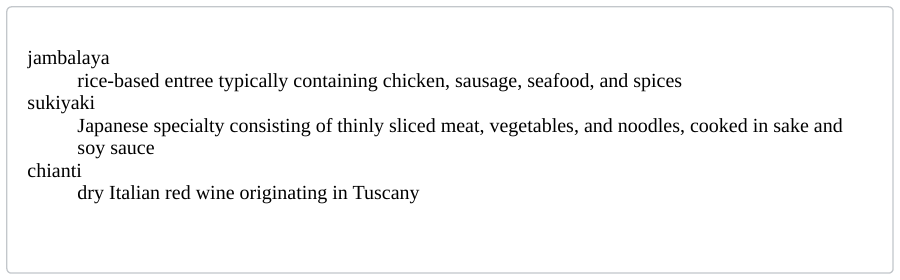
\includegraphics[width=0.92\linewidth]{figures/fig-dl-plain.png}
\end{LTR}
\caption{شکل \lr{1}. نمایش پیش‌فرض \en{description list} در مرورگر.}
\end{figure}

اگر می‌خواهید \en{keyword}ها بیشتر دیده شوند، می‌توانید پررنگشان کنید.
یادتان باشد ظاهر صفحه کارِ \en{HTML} نیست؛ برای این کار به \en{CSS} نیاز
دارید. اینجا خاصیت \en{font-weight} همان چیزی است که لازم دارید:

\begin{latin}
\begin{Verbatim}[fontsize=\small,frame=single,framesep=4pt]
dt {
  font-weight: bold;
}
\end{Verbatim}
\end{latin}

نتیجه کمی خواناتر می‌شود:

\begin{figure}[ht]
\centering
\begin{LTR}
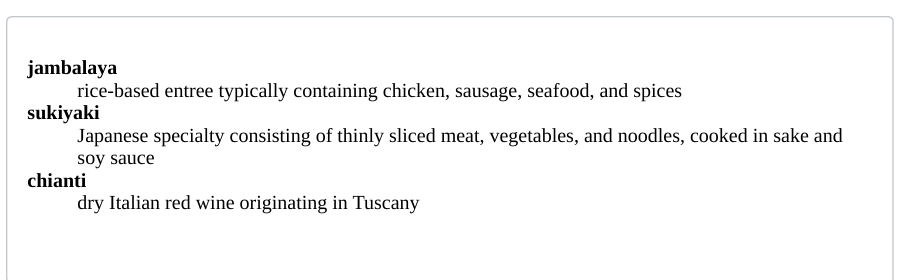
\includegraphics[width=0.92\linewidth]{figures/fig-dl-bold.png}
\end{LTR}
\caption{شکل \lr{2}. همان فهرست بعد از \en{font-weight: bold} روی
\en{dt}.}
\end{figure}

\section{بیشتر بخوانید}

\begin{itemize}
\item \en{<dfn>}
\item \en{<dl>}
\item \en{<dt>}
\item \en{<dd>}
\item چطور از \en{attribute aria-describedby} استفاده کنید
\end{itemize}

\begin{latin}
\section*{References}
\begin{itemize}
\item MDN, ``Define terms with HTML'',
  \url{https://developer.mozilla.org/en-US/docs/Web/HTML/How_to/Define_terms_with_HTML}
\end{itemize}
\end{latin}

\clearpage
\section*{یادداشت نشر}
این متن ترجمهٔ فارسی مطلبی از \en{MDN} است با عنوان انگلیسی
\begin{latin}Define terms with HTML\end{latin}.
منبع:
\en{\url{https://developer.mozilla.org/en-US/docs/Web/HTML/How_to/Define_terms_with_HTML}}
— مجوز منبع: طبق اعلام \en{MDN} (معمولاً \en{CC-BY-SA}) — تاریخ بازیابی:
\en{2026-09-14}.
ترجمه با \en{scientific-fa-translation-skill} انجام شده است.

\end{document}
